\documentclass{article}
\usepackage{amsmath}
\usepackage{amssymb}
\usepackage{esvect}
\usepackage[usenames, dvipsnames]{color}
\usepackage{fancyhdr}
\usepackage{hyperref}
\usepackage{pgfplots}
\usepackage{tikz}
\usepackage{geometry}
\usepackage[normalem]{ulem}

\geometry{letterpaper, portrait, margin=0.5in}
\pagestyle{fancy}

\fancyhf{} % clear all header fields
\renewcommand{\headrulewidth}{0pt}
\fancyfoot[LE,RO]{\thepage}           % page number in "outer" position of footer line
\fancyfoot[RE,LO]{\copyright\;aquarc 2025. \href{https://aquarc.org}{\underline{aquarc.org}}} % other info in "inner" position of footer line

\definecolor{myred1}{RGB}{255, 0, 0}
\definecolor{myyellow1}{RGB}{255, 255, 219}
\definecolor{mygreen1}{RGB}{0, 255, 0}
\definecolor{mygreen2}{RGB}{0, 126, 0}
\definecolor{myblue1}{RGB}{0, 0, 255}

\usepgfplotslibrary{polar}

\pgfplotsset{compat=1.18}
\usepgfplotslibrary{polar}
\pgfplotsset{my style polar/.append style={xticklabels={,,
$\frac{\pi}{6}$, $\frac{\pi}{3}$, $\frac{\pi}{2}$, $\frac{2\pi}{3}$,
$\frac{5\pi}{6}$, $\pi$, $\frac{7\pi}{6}$, $\frac{4\pi}{3}$,
$\frac{3\pi}{2}$, $\frac{5\pi}{3}$,$\frac{11\pi}{6}$,}, thick }}

\begin{document}

\fontsize{14}{16}\selectfont

% center the title
\begin{center}
    \textbf{\underline{Parametric and Polar Cheatsheet}}
\end{center}

\tableofcontents
\pagebreak

\section{Parametric Intro}
When you have parameters in terms of $t$ to represent $\langle x,y\rangle$ 
You represent the function as $\langle x(t),y(t)\rangle$ and the derivative as $\langle x'(t),y'(t)\rangle$.

\begin{align*}
    \frac{dy}{dx}=\frac{\frac{dy}{dt}}{\frac{dx}{dt}} \\
    \frac{d^2y}{dx^2}=\frac{d}{dx}[f'(t)]=f''(t)*\frac{dt}{dx}=\frac{\frac{d^2y}{dt^2}}{\frac{dx}{dt}}
\end{align*}
Speed:
\begin{align*}
    \Delta r = \sqrt{x'(t)^2+y'(t)^2}
\end{align*}
If there is no change in $y(t)$:
\begin{align*}
    \Delta r = \sqrt{x'(t)^2}=|x'(t)|
\end{align*}
Distance:
\begin{align*}
    r = \int{\sqrt{x'(t)^2+y'(t)^2}dt}
\end{align*}

\section{Parametric Examples}

\begin{enumerate}
    \item Find the speed, acceleration, and distance of the following:

\begin{align*}
    \vec{v} = \langle (t-1)e^{t^2},\sin(t^{1.25})\rangle \\
    \text{speed}=\sqrt{((t-1)e^{t^2})^2+\sin^2(t^{1.25})}  \\
    \text{distance}=\int{\sqrt{((t-1)e^{t^2})^2+\sin^2(t^{1.25})}}dt  
\end{align*}

    \item The parametric equation of a curve is given by $\langle 2t-1, 3t^2+1\rangle$. What is the slope of the tangent line to the curve at $t=2$. 

\begin{align*}
    \frac{dy}{dx}= \frac{\frac{dy}{dt}}{\frac{dx}{dt}} = \frac{\frac{d}{dx}[3t^2+1]}{\frac{d}{dx}[2t-1]} = \frac{6t}{2}=\frac{12}{2}=6
\end{align*}

    \item A parametric is given by $\langle \cos t, \sin t\rangle$. What is the speed of the particle  at $t=\frac{\pi}{4}$?
\begin{align*}
    \frac{dy}{dx}=\frac{\frac{dy}{dt}}{\frac{dx}{dt}} = \frac{\frac{d}{dx}[\sin t]}{\frac{d}{dx}[\cos t]} = \frac{\cos t}{-\sin t}=-1 \\
    \text{speed}=\sqrt{\cos^2 t + \sin^2 t} = 1
\end{align*}

    \item A parametric is represneted by $\langle 5t, 4-t^2\rangle$. At what value of $t$ does the curve have a horizontal tangent line?
\begin{align*}
    \frac{dy}{dt}=0=\frac{d}{dt}[4-t^2]=-2t \Longrightarrow t=0
\end{align*}

    \item A parametric is represented $\vec{v}=\langle 2t+1, 3t^2-4t\rangle$. What is the second derivative of $y$ with respect to $x$ at $t=2$?
\begin{align*}
    \frac{\vec{v}'(t)}{\frac{dx}{dt}}=\frac{\frac{6t}{2}}{2}=3
\end{align*}
\end{enumerate}

\section{Polar}
The polar axis defines functions for $r(\theta)$ where radius is the distance from $(0,0)$ and $\theta$ is the angle with the horizontal.
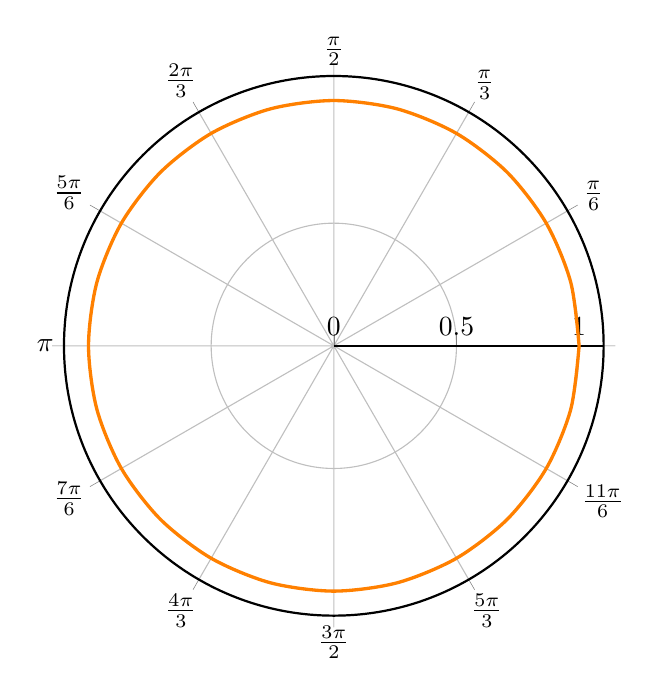
\begin{tikzpicture}
   \begin{polaraxis}[xmin=0,xmax=360,
       domain=0:360,
       my style polar,
       no markers]
       \addplot +[orange, very thick, smooth] {1};
    \end{polaraxis}
\end{tikzpicture}

A unit circle defined in Polar.

\begin{align*}
x=r\cos(\theta) \\
y=r\sin(\theta)
\end{align*}

If we were to convert the unit circle to a parametric equation we would get \\
$\langle r\cos(\theta),r\sin(\theta)\rangle$.

\subsection{Tangent Lines}
Finding tangent lines of a Polar function is quite simple; just convert it to parametric. 

Find the derivative of the following at $\frac{3 \pi}{4}$:

\begin{align*}
    r(\theta) = 4\sin(2\theta) \\
    r(\theta)cos(\theta) = 4\sin(2\theta)\cos(\theta) 
    \Longrightarrow x=4\sin(2\theta)\cos(\theta) \\
    y=4\sin(2\theta)sin(\theta) \\
    \frac{dy}{dt}=4\sin(2\theta)\cos(\theta)+8\sin(\theta)cos(2\theta) \\
    \frac{dx}{dt}=-4\sin(2\theta)\sin(\theta)+8\cos(\theta)\cos(2\theta) \\
    \frac{dy}{dx}=\frac{\sin(2\theta)\cos(\theta)+2\cos(2\theta)\sin(\theta)}
            {-\sin(2\theta)\sin(\theta)+2\cos(2\theta)\cos(\theta)} \\
    \frac{\frac{\sqrt{2}}{2}}{\frac{\sqrt{2}}{2}} = 1
\end{align*}

\subsection{Arc Length}

Using a parametric to start with:

\begin{align*}
    \text{distance}=\int{\sqrt{\biggr(\frac{dx}{dt}\biggr)^2+\biggr(\frac{dy}{dt}\biggr)^2}}dt \\
    \text{distance}=\int{\sqrt{\biggr(\frac{dr}{d\theta}r\cos\theta\biggr)^2
        +\biggr(\frac{dr}{d\theta}r\sin\theta\biggr)^2}}d\theta \\
    \text{distance}=\int{\sqrt{\biggr(-r\sin\theta+\frac{dr}{d\theta}\cos\theta)^2
        +\biggr(r\cos\theta+\frac{dr}{d\theta}\sin\theta\biggr)^2}}d\theta \\
    \Longrightarrow \int{\sqrt{r^2\sin^2\theta-2r\frac{dr}{d\theta}\sin\theta\cos\theta+
            \biggr(\frac{dr}{d\theta}\biggr)^2\cos^2\theta
        +r^2\cos^2\theta+2r\frac{dr}{d\theta}\cos\theta\sin\theta+
            \biggr(\frac{dr}{d\theta}\biggr)^2\sin^2\theta}}d\theta\\
    \Longrightarrow \int{\sqrt{r^2\sin^2\theta+
            \biggr(\frac{dr}{d\theta}\biggr)^2\cos^2\theta
        +r^2\cos^2\theta+
            \biggr(\frac{dr}{d\theta}\biggr)^2\sin^2\theta}}d\theta\\
    \Longrightarrow \int{\sqrt{r^2(\sin^2\theta+\cos^2\theta)+
            \biggr(\frac{dr}{d\theta}\biggr)^2(\cos^2\theta+\sin^2\theta)}}d\theta\\
    \Longrightarrow \int{\sqrt{r^2+
            \biggr(\frac{dr}{d\theta}\biggr)}}d\theta\\
\end{align*}

\subsection{$e^{-\theta}$}
Find arc length:
\begin{align*}
    r=e^{-\theta}=\frac{1}{e^{\theta}}
    \Longrightarrow \int_0^{\infty}{\sqrt{\biggr(\frac{1}{e^{\theta}}\biggr)^2+\biggr(\frac{-1}{e^{\theta}}\biggr)^2}}d\theta \\
    \Longrightarrow \int_0^{\infty}{\sqrt{\frac{1}{e^{2\theta}}+\frac{1}{e^{2\theta}}}}d\theta \\
    \Longrightarrow \int_0^{\infty}{\sqrt{\frac{2}{e^{2\theta}}}}d\theta
    \Longrightarrow \sqrt{2}\int_0^{\infty}{\sqrt{\frac{1}{e^{2\theta}}}}d\theta
    \Longrightarrow \sqrt{2}\int_0^{\infty}{(\frac{1}{e^{2\theta}})^{\frac{1}{2}}}d\theta
    \Longrightarrow \sqrt{2}\int_0^{\infty}{e^{-\theta}}d\theta
    \Longrightarrow -\sqrt{2}e^{-\theta}\biggr\rvert^{\infty}_{0}\\
    =\sqrt{2}
\end{align*}

\subsection{Area in the Curve}
A polar graph can be thought in terms of mini-sectors in the way an integral is thought of in rectangles.

\begin{align*}
    A_{\text{arc}}=\frac{\theta}{2\pi}\pi r^2
    =\frac{1}{2}r^2\theta \\
    A_{r(\theta)}=\int{\frac{1}{2}r^2d\theta}
\end{align*}

\subsection{Examples}

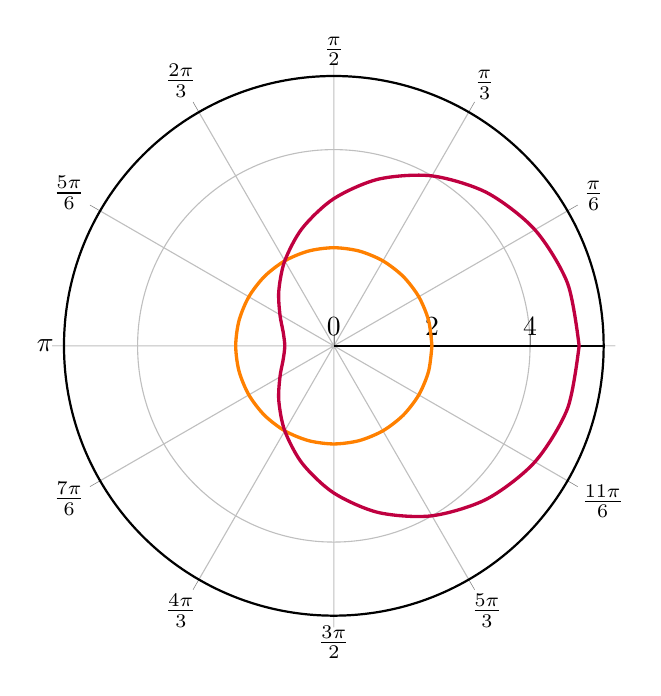
\begin{tikzpicture}
   \begin{polaraxis}[xmin=0,xmax=360,
       domain=0:360,
       my style polar,
       no markers]
       \addplot +[orange, very thick, smooth] {2};
       \addplot +[purple, very thick, smooth] {3 + 2 * cos(x)};
    \end{polaraxis}
\end{tikzpicture}

Find the area inside.

\begin{align*}
    A=\frac{\pi 2^2}{2}+\frac{1}{2}\int_{\frac{\pi}{2}}^{\frac{3\pi}{2}}{(3+2\cos\theta)^2}d\theta
\end{align*}

\end{document}
